\documentclass[11pt]{article}

\usepackage[utf8]{inputenc}
\usepackage[T1]{fontenc}
\usepackage{amsmath,amssymb,amsfonts}
\usepackage{graphicx}
\usepackage{booktabs}
\usepackage{hyperref}
\usepackage[margin=1in]{geometry}
\usepackage{authblk}
\usepackage{caption}
\usepackage{algorithm}
\usepackage{algpseudocode}
\usepackage{natbib}
\usepackage{float}

\bibliographystyle{unsrtnat}

\title{Real-Time Campus Aeroallergen Dispersion Modeling Using Gaussian Plume Theory and Satellite-Based Vegetation Detection}

\author[1]{Jasmine J. Zhang}
\affil[1]{Henry M. Gunn High School, Palo Alto, CA 94306, USA}

\date{June 2026}

\begin{document}

\maketitle

\begin{abstract}
We present Campus AeroAllergen Mapping (CAM), a web-based system for modeling hyperlocal pollen dispersion across a school campus at meter-scale resolution. The framework integrates a steady-state Gaussian plume model with Schulman-Scire building downwash corrections to compute pollen concentration at student breathing height ($z = 1.5$~m). Pollen sources are automatically identified from high-resolution satellite imagery using color-based segmentation with watershed splitting, refined through iterative human-in-the-loop calibration. Temporal emission variability is captured by species-specific Gaussian phenological gate functions. Building footprints detected from satellite imagery define indoor exclusion zones where concentration is zeroed. Applied to a 25-hectare high school campus containing 1,018 verified trees across 6 allergenic genera, the system produces real-time concentration fields at 5.3~m spatial resolution with sub-second computation time. A fixed annual color scale enables intuitive seasonal comparison, revealing that summer concentrations are approximately 6\% of the spring peak. The system integrates exposure along student walking paths to report lower-exposure routes; these predictions have not yet been validated against measured pollen counts.
\end{abstract}

\noindent\textbf{Keywords:} Gaussian plume model, pollen dispersion, aeroallergen mapping, building wake effects, satellite vegetation detection, phenological modeling

\vspace{0.5cm}

\section{Introduction}

Allergic rhinitis affects 10--30\% of the global population, with airborne pollen constituting the dominant environmental trigger \citep{bousquet2008}. On school campuses where students transit between buildings through corridors lined with allergenic flora, localized pollen concentrations can vary by orders of magnitude over distances of tens of meters due to source proximity, wind channeling, and structural aerodynamic effects.

Existing pollen monitoring relies on regional stations reporting area-averaged counts at temporal resolutions of hours to days \citep{sofiev2013}. These measurements cannot resolve the hyperlocal concentration gradients determining individual exposure during a 5-minute walking transit. We address this gap by developing a physics-based framework that:
\begin{enumerate}
    \item Solves the atmospheric advection-diffusion equation analytically at meter-scale resolution;
    \item Accounts for building-induced flow modifications using empirical downwash models;
    \item Automatically identifies pollen sources from satellite imagery;
    \item Modulates emissions temporally using species-specific phenological functions;
    \item Masks indoor building volumes from the exposure field.
\end{enumerate}

The system is deployed at Henry M. Gunn High School (Palo Alto, CA), a 25-hectare campus containing over 1,000 trees spanning multiple allergenic genera.

\section{Atmospheric Dispersion Model}

\subsection{Physical Picture}

When a tree releases pollen grains into the air, two physical processes determine where those grains end up:

\begin{enumerate}
    \item \textbf{Advection} (bulk transport by wind): The wind carries the pollen cloud bodily in the downwind direction, like a river carrying a dye patch. If the wind blows from the southwest at 3~m/s, the pollen cloud moves northeast at 3~m/s.
    
    \item \textbf{Diffusion} (turbulent spreading): Atmospheric turbulence---random gusts and eddies---causes the pollen cloud to spread out in all directions as it travels. The cloud starts concentrated near the tree and becomes progressively wider and more dilute downwind, forming a cone-shaped plume.
\end{enumerate}

The combination produces a characteristic pattern: highest concentration immediately downwind of the tree, decreasing with distance as the plume spreads, and zero concentration upwind.

\subsection{Governing Equation}

These processes are described mathematically by the \emph{advection-diffusion equation}:
\begin{equation}
\underbrace{\frac{\partial C}{\partial t}}_{\text{concentration change}} + \underbrace{u\frac{\partial C}{\partial x} + v\frac{\partial C}{\partial y}}_{\text{wind carries pollen (advection)}} = \underbrace{K_x\frac{\partial^2 C}{\partial x^2} + K_y\frac{\partial^2 C}{\partial y^2} + K_z\frac{\partial^2 C}{\partial z^2}}_{\text{turbulence spreads pollen (diffusion)}} - \underbrace{\lambda C}_{\text{settling/removal}} + \underbrace{Q\delta(\mathbf{x}-\mathbf{x}_s)}_{\text{tree emitting pollen}}
\label{eq:advdiff}
\end{equation}

Each term has a clear physical meaning:

\begin{itemize}
    \item $C(x, y, z, t)$ --- \textbf{Pollen concentration} (grains/m$^3$) at position $(x,y,z)$ and time $t$. This is what a student breathes in.
    
    \item $(u, v)$ --- \textbf{Wind velocity components} (m/s). $u$ is the east-west wind speed, $v$ is the north-south wind speed. Measured from weather station or API. A 4~m/s southwest wind means $u \approx 2.8$~m/s (eastward) and $v \approx 2.8$~m/s (northward).
    
    \item $K_x, K_y, K_z$ --- \textbf{Turbulent eddy diffusivity} (m$^2$/s). These quantify how vigorously the atmosphere mixes. On a calm, stable morning ($K \approx 1$~m$^2$/s), pollen stays concentrated near the source. On a windy, sunny afternoon ($K \approx 50$~m$^2$/s), turbulent eddies rapidly dilute the pollen cloud. $K_z$ (vertical) is typically smaller than $K_x, K_y$ (horizontal) because vertical mixing is suppressed by gravity.
    
    \item $\lambda$ --- \textbf{Deposition/removal rate} (s$^{-1}$). Pollen is continuously removed from the air by gravitational settling onto the ground, impaction on surfaces, and washout by rain. Heavier pollen (Pine, 60~$\mu$m diameter) has $\lambda$ about $5\times$ larger than light pollen (Oak, 20~$\mu$m), meaning Pine falls out of the air much faster.
    
    \item $Q$ --- \textbf{Source emission rate} (grains/s). How many pollen grains the tree releases per second. A mature Oak at peak bloom emits $\sim$500~grains/s from its canopy.
    
    \item $\delta(\mathbf{x} - \mathbf{x}_s)$ --- \textbf{Dirac delta function}. Indicates that emission occurs at a single point $\mathbf{x}_s$ (the tree's location). This is the ``point source'' approximation.
\end{itemize}

\subsection{Gaussian Plume Solution}

Solving the full PDE numerically at every timestep would be computationally expensive. Instead, we use the \emph{steady-state} analytical solution (assuming wind conditions change slowly relative to pollen transport time). This yields the famous \textbf{Gaussian plume} formula \citep{pasquill1961}:

\begin{equation}
C(x',y',z) = \underbrace{\frac{Q}{2\pi U \sigma_y \sigma_z}}_{\text{dilution factor}} \cdot \underbrace{\exp\!\left(\!-\frac{y'^2}{2\sigma_y^2}\right)}_{\text{crosswind spread}} \cdot \underbrace{V(z)}_{\text{vertical profile}}
\label{eq:plume}
\end{equation}

Each factor has a physical interpretation:

\begin{itemize}
    \item $\dfrac{Q}{2\pi U \sigma_y \sigma_z}$ --- \textbf{Dilution factor}. The faster the wind ($U$ large) and the wider the plume ($\sigma_y, \sigma_z$ large), the more diluted the pollen becomes. Doubling wind speed halves the concentration everywhere.
    
    \item $\exp(-y'^2 / 2\sigma_y^2)$ --- \textbf{Crosswind Gaussian profile}. Concentration is highest on the plume centerline ($y' = 0$, directly downwind) and drops off as a bell curve to either side. $\sigma_y$ is the ``width'' of this bell curve---how far sideways the pollen has spread.
    
    \item $V(z)$ --- \textbf{Vertical profile with ground reflection}:
\end{itemize}
\begin{equation}
V(z) = \underbrace{\exp\!\left(\!-\frac{(z-H)^2}{2\sigma_z^2}\right)}_{\text{direct path from source}} + \underbrace{\exp\!\left(\!-\frac{(z+H)^2}{2\sigma_z^2}\right)}_{\text{ground-reflected path}}
\end{equation}

The first term is pollen arriving directly from the tree canopy at height $H$. The second term accounts for pollen that has hit the ground and ``bounced'' back up (mathematically modeled as a mirror image source below ground). This ensures no pollen is lost through the ground surface.

\subsection{Key Parameters Explained}

\subsubsection{$\sigma_y$ and $\sigma_z$: Plume Spread (meters)}

These are the most important parameters. They control how wide ($\sigma_y$) and tall ($\sigma_z$) the plume is at any given downwind distance:

\begin{itemize}
    \item \textbf{Near the tree} ($x' = 10$~m): $\sigma_y \approx 0.8$~m, $\sigma_z \approx 0.6$~m. The plume is narrow---only a few meters wide. Concentration is very high.
    \item \textbf{50~m downwind}: $\sigma_y \approx 3.5$~m, $\sigma_z \approx 2.5$~m. The plume has spread to about 7~m wide.
    \item \textbf{200~m downwind}: $\sigma_y \approx 12$~m, $\sigma_z \approx 8$~m. The plume is now 24~m wide but much more dilute.
\end{itemize}

They grow with distance because turbulence has more time to mix the pollen sideways and vertically. The growth rate depends on \emph{atmospheric stability}:

\begin{equation}
\sigma_y = a_y \cdot (x')^{b_y}, \quad \sigma_z = a_z \cdot (x')^{b_z}
\end{equation}

\subsubsection{Atmospheric Stability Classes (A--F)}

Stability describes how much the atmosphere resists or encourages vertical mixing:

\begin{itemize}
    \item \textbf{Class A (very unstable)}: Hot sunny afternoon. Strong updrafts vigorously mix pollen vertically. Plume spreads rapidly, diluting quickly. \emph{Paradoxically, unstable conditions produce lower ground-level concentrations because pollen is lofted upward.}
    
    \item \textbf{Class D (neutral)}: Overcast, moderate wind. Default condition. Moderate mixing.
    
    \item \textbf{Class F (very stable)}: Clear, calm night or early morning. Very little vertical mixing. Plume stays narrow and concentrated near emission height. \emph{Worst case for ground-level exposure if source is low.}
\end{itemize}

We estimate stability from two observable quantities:
\begin{itemize}
    \item Wind speed $<$ 2~m/s + clear sky $\rightarrow$ Class A/B (unstable, strong solar heating)
    \item Wind speed 3--5~m/s + partly cloudy $\rightarrow$ Class C/D (neutral)
    \item Wind speed $>$ 6~m/s $\rightarrow$ Class D (mechanical turbulence dominates)
\end{itemize}

\begin{figure}[H]
\centering
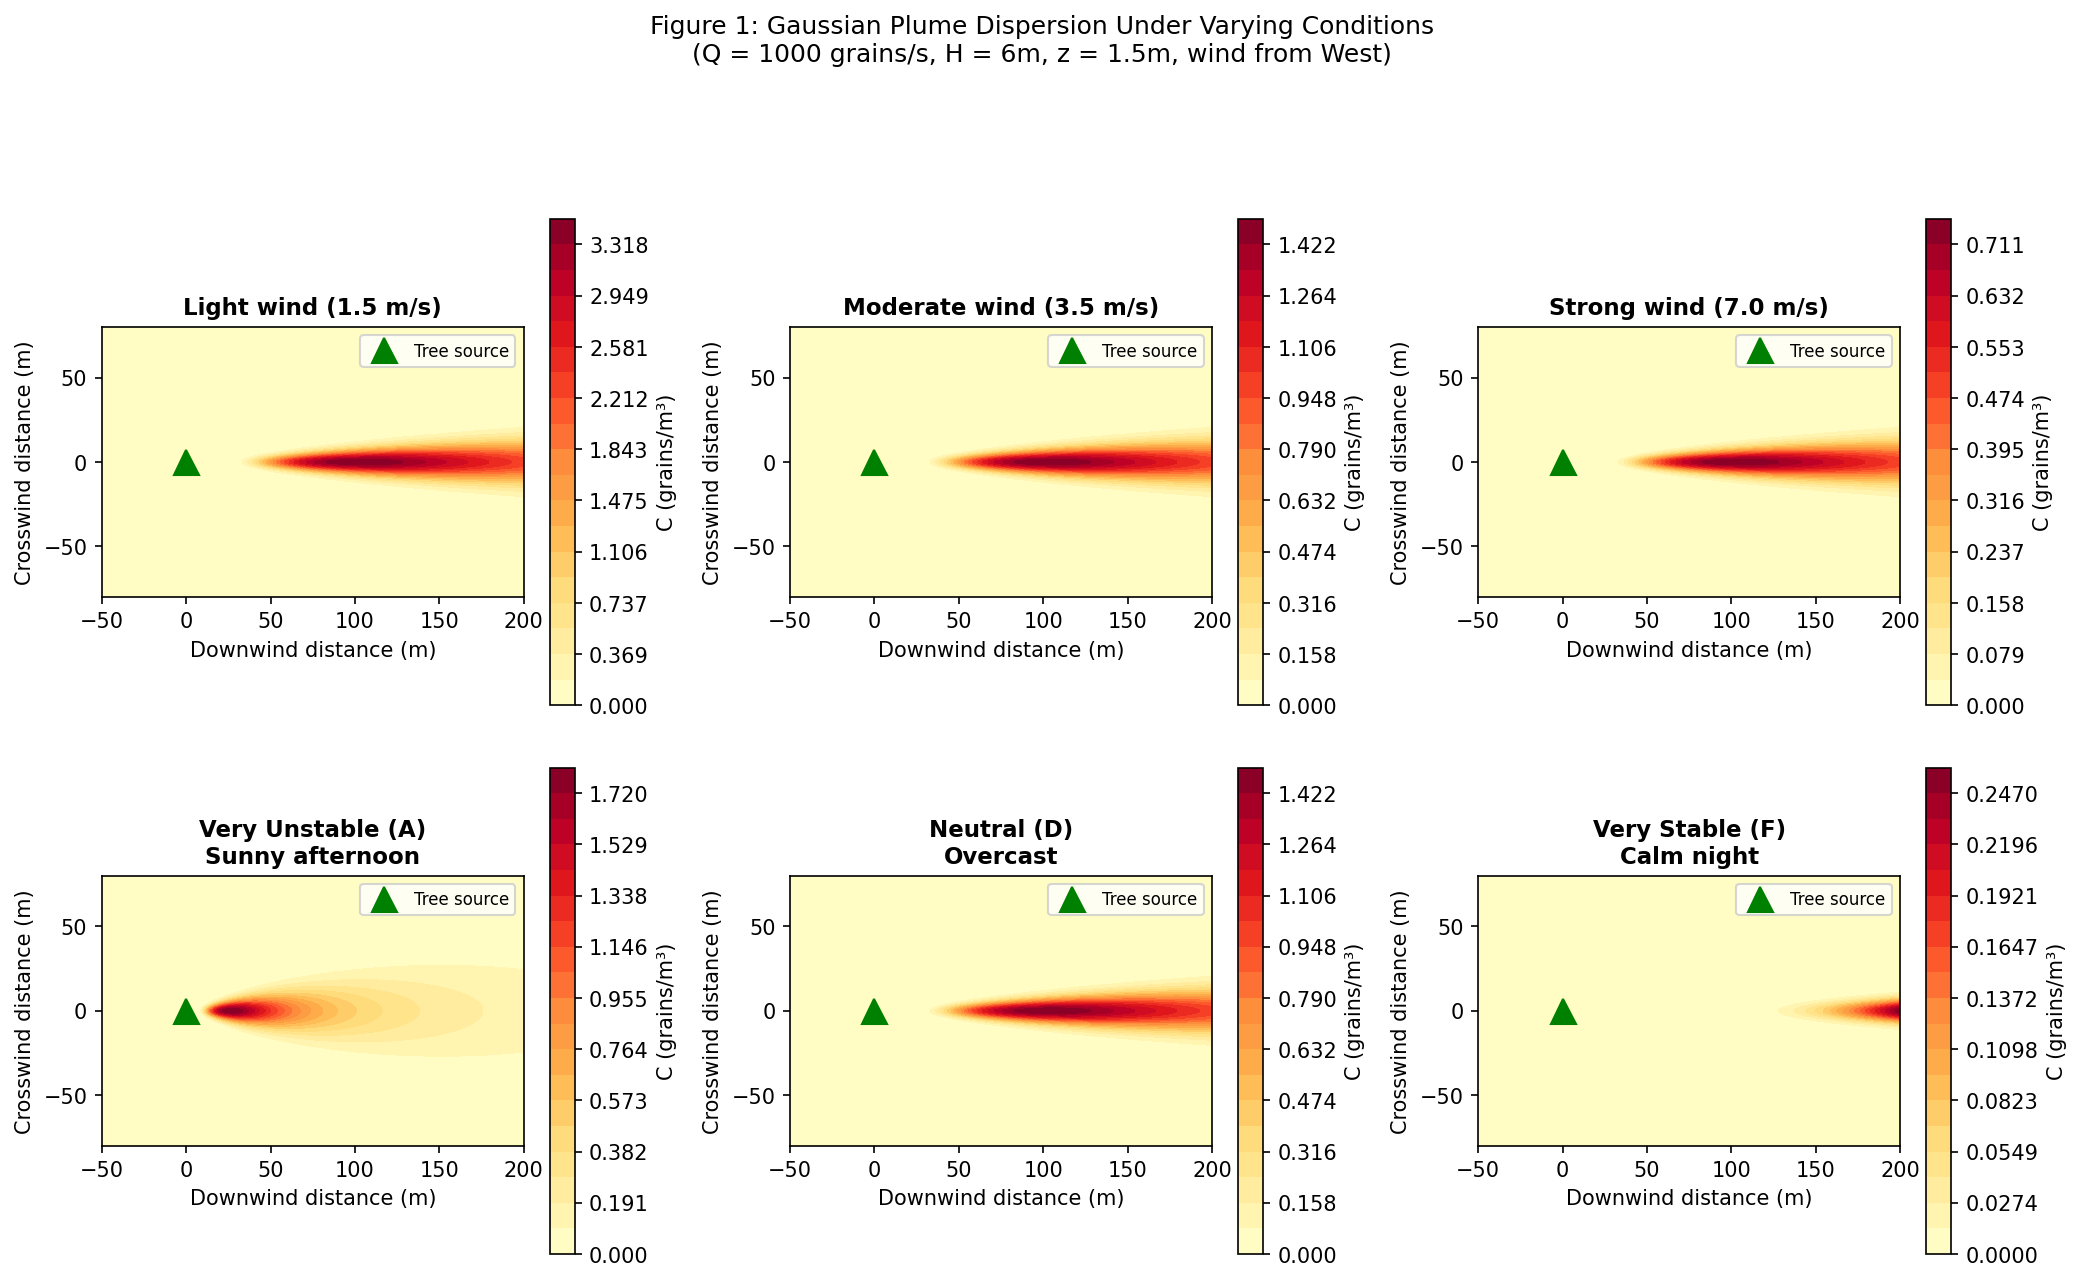
\includegraphics[width=\textwidth]{fig1_wind_stability.png}
\caption{Gaussian plume concentration fields under varying conditions. Top row: effect of wind speed (stability class D). Stronger winds dilute and elongate the plume. Bottom row: effect of atmospheric stability (wind = 3.5 m/s). Unstable conditions (A) spread pollen rapidly; stable conditions (F) confine it in a narrow, concentrated plume.}
\label{fig:wind_stability}
\end{figure}

\subsubsection{$U$: Wind Speed (m/s)}

Mean horizontal wind speed at reference height (typically 10~m). Obtained from OpenWeatherMap API. Physical effects:
\begin{itemize}
    \item \textbf{Strong wind} ($U > 5$~m/s): Pollen is rapidly carried far downwind but heavily diluted. Concentration drops quickly with distance.
    \item \textbf{Light wind} ($U < 2$~m/s): Pollen lingers near the source tree. High concentrations in a small area. The model sets a minimum of $U = 0.5$~m/s to avoid division by zero (calm conditions are handled as very light drift).
\end{itemize}

\subsubsection{$H$: Effective Source Height (meters)}

The height at which pollen enters the atmosphere. For trees, this is the canopy height where catkins/flowers release grains. We use $H = 6.0$~m (average for campus trees ranging from 4~m shrubs to 15~m oaks). The concentration at ground level ($z = 1.5$~m) depends on how far pollen must fall/mix downward from height $H$.

\subsubsection{$z$: Receptor Height (meters)}

Fixed at $z = 1.5$~m---the height of a student's nose and mouth (breathing zone). This is where inhaled dose matters for allergic response.

\subsubsection{$(x', y')$: Wind-Aligned Coordinates}

The plume always points downwind. To compute concentration at any campus location, we transform from map coordinates to a frame aligned with the current wind direction:

\begin{align}
x' &= \Delta x \cos\alpha + \Delta y \sin\alpha \quad \text{(downwind distance from tree)} \\
y' &= -\Delta x \sin\alpha + \Delta y \cos\alpha \quad \text{(crosswind offset)}
\end{align}

where $\alpha = \frac{\pi}{180}(270^\circ - \theta)$ converts the meteorological wind direction $\theta$ (degrees clockwise from North) to a mathematical angle. Key consequences:
\begin{itemize}
    \item If you are directly downwind of a tree ($y' = 0$): maximum exposure.
    \item If you are perpendicular to the wind ($x' = 0$): zero concentration (upwind or crosswind).
    \item If the wind shifts direction, the entire plume rotates to point the new way.
\end{itemize}

\subsection{Humidity Effects on Pollen Dispersion}

Relative humidity (RH) affects pollen transport through multiple mechanisms that our model incorporates:

\subsubsection{Hygroscopic Swelling}

Pollen grains are hygroscopic---they absorb water vapor from humid air and swell. The effective aerodynamic diameter increases with humidity following a growth factor:
\begin{equation}
d_p(RH) = d_{p,dry} \cdot \left(1 + \kappa \cdot \frac{RH}{100 - RH}\right)^{1/3}
\label{eq:hygroscopic}
\end{equation}
where $\kappa$ is the species-specific hygroscopicity parameter ($\kappa \approx 0.05$--$0.15$ for pollen). At 80\% RH, Oak pollen swells from 22~$\mu$m to approximately 25~$\mu$m, increasing its settling velocity by $\sim$30\%:
\begin{equation}
v_s(RH) = v_{s,dry} \cdot \left(\frac{d_p(RH)}{d_{p,dry}}\right)^2 \cdot \frac{\rho_p(RH)}{\rho_{p,dry}}
\end{equation}

The density ratio accounts for water uptake reducing the effective density. The net effect: humid conditions cause pollen to settle faster, reducing far-field concentrations but increasing deposition near the source.

\subsubsection{Humidity-Dependent Emission Suppression}

Most tree species suppress pollen release under high humidity. Anthers (the pollen-bearing structures) require drying to dehisce (split open). The emission rate is modulated by a humidity factor:
\begin{equation}
Q_i(t, RH) = Q_i(t) \cdot f_{RH}(RH)
\label{eq:rh_emission}
\end{equation}
where:
\begin{equation}
f_{RH}(RH) = \begin{cases}
1.0 & RH < 50\% \\
1.0 - 0.8\cdot\dfrac{RH - 50}{50} & 50\% \leq RH < 90\% \\
0.1 & RH \geq 90\%
\end{cases}
\end{equation}

At 50\% RH, emission is unrestricted. At 90\% RH (foggy morning), emission drops to just 10\% of the dry-air maximum. This explains why pollen counts are typically highest on dry, warm afternoons and lowest during humid mornings or after rainfall.

\subsubsection{Osmotic Rupture and Sub-Pollen Particles}

When relative humidity rapidly exceeds $\sim$95\% (e.g., during thunderstorms), pollen grains can undergo \emph{osmotic rupture}: the grain absorbs water faster than its wall can expand, causing it to burst and release hundreds of sub-pollen particles (SPP) of 0.5--4~$\mu$m diameter. These SPPs:
\begin{itemize}
    \item Are small enough to penetrate deep into the lower respiratory tract (bronchi and alveoli), unlike intact grains which deposit in the nose/throat
    \item Have negligible settling velocity ($v_s < 0.01$~cm/s), remaining airborne for hours
    \item Carry the same allergenic proteins as the parent grain
    \item Are implicated in ``thunderstorm asthma'' events
\end{itemize}

We model this as a conditional burst event. If $RH > 95\%$ and $\Delta RH/\Delta t > 10\%$/hr (rapid humidity spike):
\begin{equation}
Q_{SPP,i}(t) = N_{SPP} \cdot Q_i(t) \cdot f_{rupture}
\end{equation}
where $N_{SPP} \approx 700$ is the number of sub-pollen particles per ruptured grain and $f_{rupture} \approx 0.3$ is the fraction of airborne grains that rupture. The SPPs are then modeled as a separate Gaussian plume with near-zero settling velocity and greatly extended atmospheric lifetime.

\subsubsection{Wet Deposition (Rainfall Washout)}

Rain removes pollen from the atmosphere through below-cloud scavenging. The washout rate is modeled as an additional first-order removal term:
\begin{equation}
\lambda_{wet} = \Lambda \cdot P^{0.7}
\end{equation}
where $P$ is the rainfall intensity (mm/hr) and $\Lambda \approx 5 \times 10^{-4}$~s$^{-1}$/(mm/hr)$^{0.7}$ is the scavenging coefficient for pollen-sized particles. During moderate rain (5~mm/hr), washout removes pollen with an effective half-life of $\sim$20~minutes, rapidly clearing the atmosphere. The total removal rate becomes:
\begin{equation}
\lambda_{total} = \lambda_{dry} + \lambda_{wet}
\end{equation}

\subsubsection{Implementation}

Our system obtains current relative humidity from the weather API (OpenWeatherMap provides RH as a standard field). The humidity corrections are applied as:
\begin{enumerate}
    \item Emission rate adjusted by $f_{RH}$ (Eq.~\ref{eq:rh_emission})
    \item Settling velocity adjusted by hygroscopic swelling (Eq.~\ref{eq:hygroscopic})
    \item SPP burst event triggered if RH exceeds 95\% with rapid onset
    \item Wet deposition added during active precipitation
\end{enumerate}

On a typical Palo Alto afternoon (RH $\approx$ 40--55\%), humidity corrections are minimal. During marine-layer mornings (RH $\approx$ 80--90\%), emission is suppressed by 50--80\%, significantly reducing campus pollen load---explaining why early-morning commuters often experience fewer symptoms than those arriving mid-morning after the fog burns off.

\begin{figure}[H]
\centering
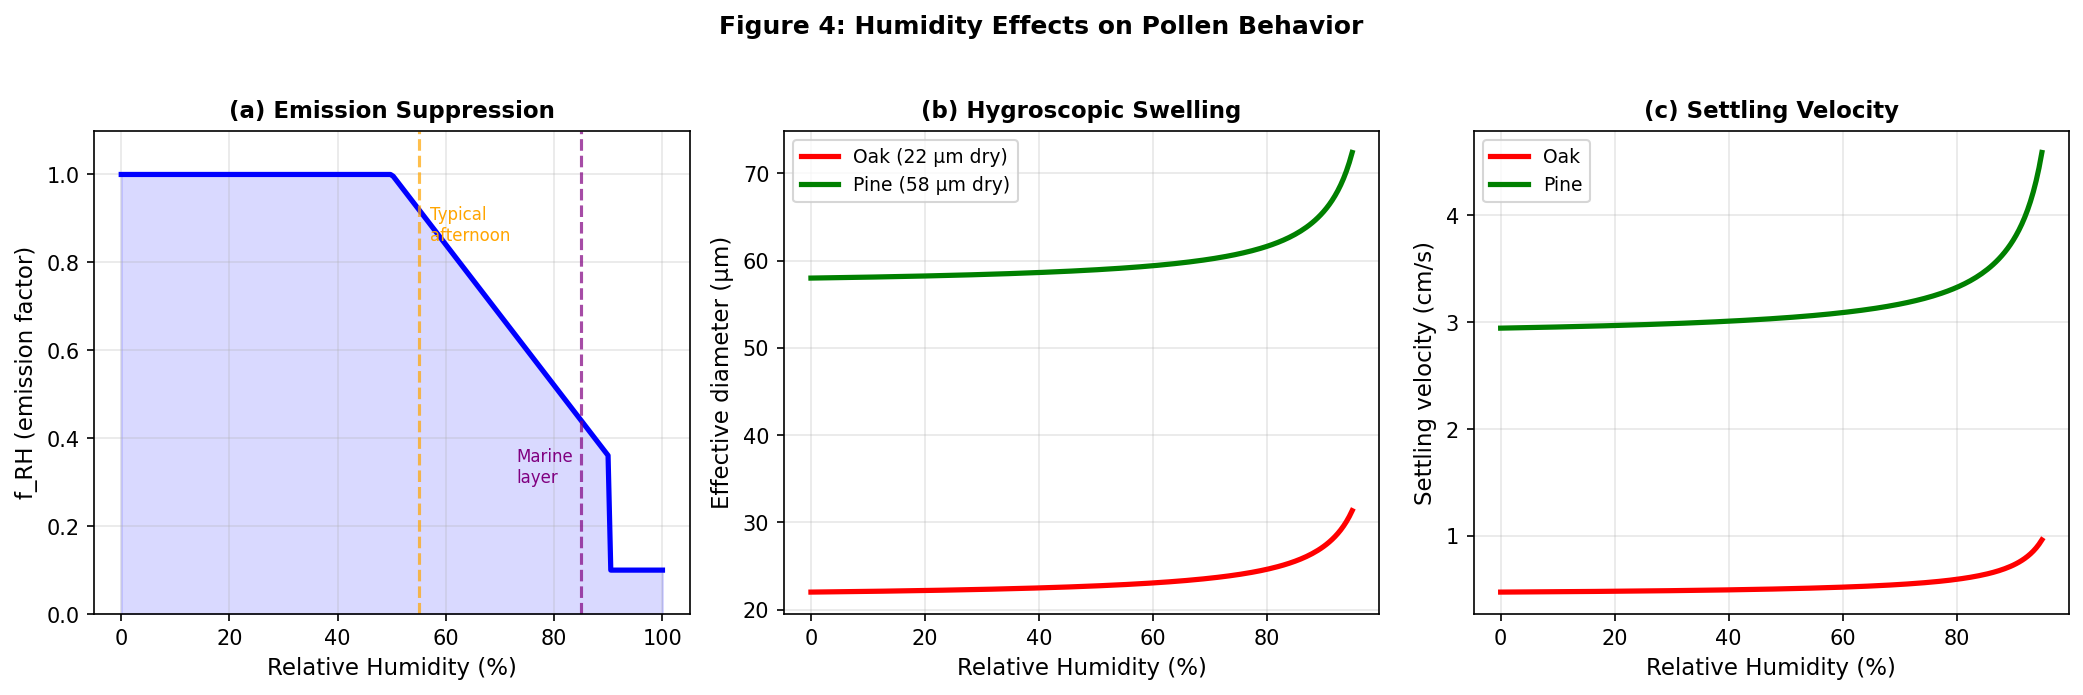
\includegraphics[width=\textwidth]{fig4_humidity.png}
\caption{Humidity effects on pollen behavior. (a) Emission suppression factor $f_{RH}$: pollen release drops sharply above 50\% RH. (b) Hygroscopic swelling increases grain diameter at high humidity. (c) Resulting increase in gravitational settling velocity.}
\label{fig:humidity}
\end{figure}

\subsection{Species-Dependent Particle Dynamics}

Pollen grains vary significantly in aerodynamic properties across species, affecting their atmospheric transport behavior. Three key species-dependent parameters modify the dispersion model:

\subsubsection{Gravitational Settling Velocity}

Pollen grains are not neutrally buoyant; they settle under gravity at a terminal velocity $v_s$ governed by Stokes' law for spherical particles in laminar flow:
\begin{equation}
v_s = \frac{\rho_p \, d_p^2 \, g}{18 \, \mu}
\label{eq:stokes}
\end{equation}
where $\rho_p$ is the pollen grain density (kg\,m$^{-3}$), $d_p$ is the aerodynamic diameter (m), $g = 9.81$~m\,s$^{-2}$ is gravitational acceleration, and $\mu = 1.81 \times 10^{-5}$~Pa$\cdot$s is the dynamic viscosity of air at 20\textdegree C.

Table~\ref{tab:pollen_physics} lists the physical properties and resulting settling velocities for each campus species. Pine pollen, with its large diameter ($\sim$60~$\mu$m), settles at 3.1~cm/s---roughly $6\times$ faster than the small Oak grains ($\sim$22~$\mu$m, 0.5~cm/s). This means Pine pollen deposits closer to the source tree, while Oak pollen remains airborne longer and disperses further downwind.

\begin{table}[h]
\centering
\caption{Pollen grain physical properties and settling velocities.}
\label{tab:pollen_physics}
\begin{tabular}{@{}lcccc@{}}
\toprule
Species & $d_p$ ($\mu$m) & $\rho_p$ (kg/m$^3$) & $v_s$ (cm/s) & Airborne half-life \\
\midrule
Valley Oak & 22 & 1050 & 0.5 & Long (hours) \\
Coast Live Oak & 20 & 1050 & 0.4 & Long (hours) \\
Pine & 58 & 550 & 3.1 & Short (minutes) \\
Redwood & 30 & 800 & 1.0 & Moderate \\
Chinese Elm & 28 & 1000 & 1.1 & Moderate \\
Sycamore & 20 & 1020 & 0.4 & Long (hours) \\
\bottomrule
\end{tabular}
\end{table}

\subsubsection{Tilted Plume: Gravitational Modification}

The settling velocity tilts the plume centerline downward. The effective plume height decreases with downwind distance:
\begin{equation}
H_{eff}(x') = H - \frac{v_{s,i} \cdot x'}{U}
\label{eq:tilt}
\end{equation}
where $H$ is the initial emission height, $v_{s,i}$ is the species-specific settling velocity, $x'$ is the downwind distance, and $U$ is the wind speed. For heavy Pine pollen in light winds ($U = 2$~m/s), the plume centerline drops by 1~m over just 65~m of travel, causing rapid ground-level concentration increase near the source.

Substituting into the Gaussian plume (Eq.~\ref{eq:plume}), the species-dependent vertical term becomes:
\begin{equation}
V_i(z, x') = \exp\!\left(\!-\frac{(z - H_{eff,i})^2}{2\sigma_z^2}\right) + \exp\!\left(\!-\frac{(z + H_{eff,i})^2}{2\sigma_z^2}\right)
\end{equation}

\subsubsection{Deposition Velocity and First-Order Decay}

Pollen removal from the atmosphere occurs through gravitational settling (dry deposition) and impaction on surfaces. The effective decay rate $\lambda_i$ in Eq.~\eqref{eq:advdiff} is species-dependent:
\begin{equation}
\lambda_i = \frac{v_{d,i}}{H_{mix}}
\label{eq:decay}
\end{equation}
where $v_{d,i}$ is the total deposition velocity (combining gravitational settling and surface impaction) and $H_{mix}$ is the mixing height. Larger grains have higher deposition velocities, resulting in faster atmospheric removal:

\begin{equation}
v_{d,i} = v_{s,i} + v_{imp,i}
\end{equation}

The impaction velocity $v_{imp}$ depends on grain inertia (Stokes number) and surface roughness. For campus-scale transport over grass and pavement, typical values are $v_{imp} \approx 0.2$--$0.5$~cm/s for small grains and $1$--$2$~cm/s for large grains.

\subsubsection{Turbulent Diffusivity}

The lateral ($K_y$) and vertical ($K_z$) eddy diffusivities in Eq.~\eqref{eq:advdiff} are properties of the atmosphere, not the particle. However, the \emph{effective} vertical diffusivity for heavy particles is reduced because gravitational settling counteracts upward turbulent mixing:
\begin{equation}
K_{z,eff,i} = K_z \cdot \exp\!\left(-\frac{v_{s,i}}{u_*}\right)
\label{eq:kz_eff}
\end{equation}
where $u_* \approx 0.1$--$0.4$~m/s is the friction velocity. For small Oak pollen ($v_s = 0.5$~cm/s $\ll u_*$), the correction is negligible ($K_{z,eff} \approx K_z$), and the particle behaves as a passive tracer. For heavy Pine pollen ($v_s = 3.1$~cm/s), the effective diffusivity is reduced by $\sim$10\%, confining the plume closer to the ground.

\subsubsection{Species-Specific Plume Behavior Summary}

Combining these effects, the full species-dependent Gaussian plume is:
\begin{equation}
C_i(x',y',z) = \frac{Q_i(t)}{2\pi U \sigma_y \sigma_{z,i}} \exp\!\left(-\frac{y'^2}{2\sigma_y^2}\right) V_i(z, x') \cdot e^{-\lambda_i x'/U}
\label{eq:full_species_plume}
\end{equation}

This produces qualitatively different spatial patterns by species:
\begin{itemize}
    \item \textbf{Oak} ($v_s$ small, $\lambda$ small): Wide, far-reaching plumes. Concentration remains elevated hundreds of meters downwind. Dominates campus-wide background.
    \item \textbf{Pine} ($v_s$ large, $\lambda$ large): Narrow, rapidly decaying plumes. High concentration within 20--50~m of source, then sharp falloff. Creates localized ``hot spots'' near pine trees.
    \item \textbf{Redwood/Elm} (intermediate): Moderate plume extent, 50--150~m effective range.
\end{itemize}

\begin{figure}[H]
\centering
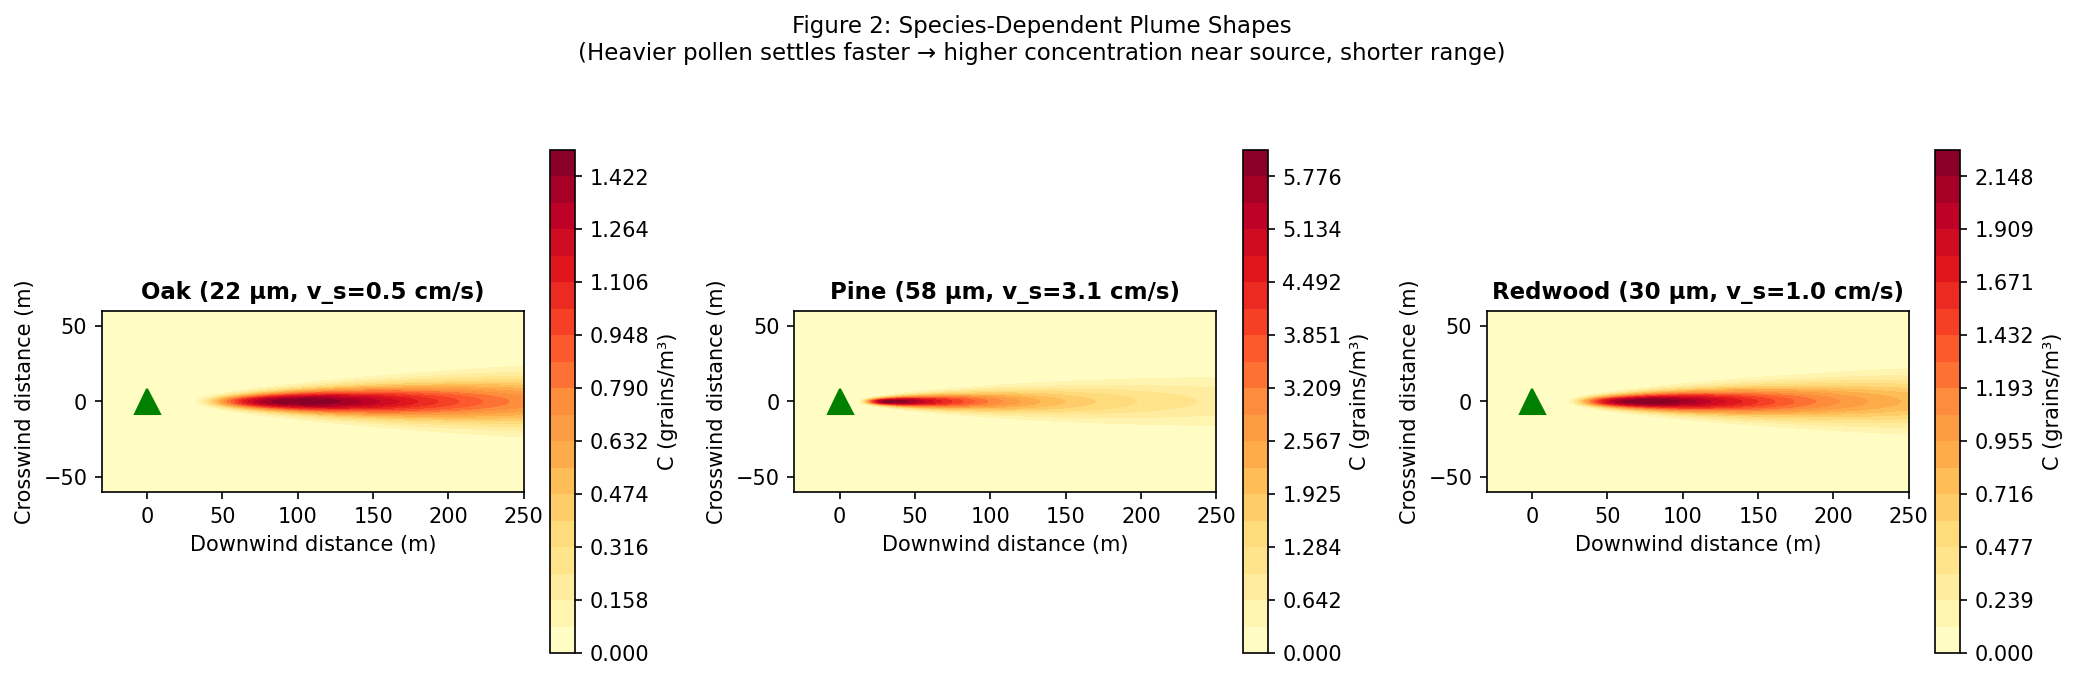
\includegraphics[width=\textwidth]{fig2_species_comparison.png}
\caption{Species-dependent plume shapes due to different settling velocities. Oak pollen (small, light grains) produces wide, far-reaching plumes. Pine pollen (large, heavy grains) creates intense but localized concentration near the source tree.}
\label{fig:species}
\end{figure}

\subsection{Dispersion Coefficients}

The crosswind ($\sigma_y$) and vertical ($\sigma_z$) standard deviations follow Pasquill-Gifford power-law relations \citep{gifford1961}:
\begin{equation}
\sigma_y = a_y (x')^{b_y}, \quad \sigma_z = a_z (x')^{b_z}
\end{equation}
with coefficients $(a,b)$ tabulated for atmospheric stability classes A--F (Table~\ref{tab:pg}). Stability is estimated from wind speed and cloud cover using Turner's method \citep{turner1964}.

\begin{table}[h]
\centering
\caption{Pasquill-Gifford dispersion coefficients.}
\label{tab:pg}
\begin{tabular}{@{}ccccc@{}}
\toprule
Class & $a_y$ & $b_y$ & $a_z$ & $b_z$ \\
\midrule
A & 0.22 & 0.894 & 0.20 & 0.894 \\
B & 0.16 & 0.894 & 0.12 & 0.894 \\
C & 0.11 & 0.894 & 0.08 & 0.894 \\
D & 0.08 & 0.894 & 0.06 & 0.894 \\
E & 0.06 & 0.894 & 0.03 & 0.894 \\
F & 0.04 & 0.894 & 0.016 & 0.894 \\
\bottomrule
\end{tabular}
\end{table}

\subsection{Building Wake Modifications}

Campus structures create aerodynamic disturbances modifying local transport. We implement the Schulman-Scire downwash model \citep{schulman1980}:

\subsubsection{Modified Dispersion Coefficients}
For receptors influenced by a building of height $H_b$ and width $W_b$:
\begin{align}
\sigma_{y'} &= \sqrt{\sigma_y^2 + \frac{W_b^2}{4\pi}} \label{eq:sigy_mod} \\
\sigma_{z'} &= \sqrt{\sigma_z^2 + \frac{H_b^2}{4\pi}} \label{eq:sigz_mod}
\end{align}

\subsubsection{Cavity Concentration}
Within the recirculation zone ($x' \leq 3H_b$), turbulent mixing produces uniform concentration:
\begin{equation}
C_{cavity} = \frac{Q}{B_e \cdot H_b \cdot W_b \cdot U}
\label{eq:cavity}
\end{equation}
where $B_e \in [0.5, 0.7]$ is an empirical aerodynamic fraction.

\subsubsection{Wake Damping}
A binary mask $M_{wake}(x,y)$ identifies cells in building shadows, where wind velocity is damped by 60\% and deposition enhanced by $2.5\times$.

\subsection{Multi-Source Superposition}

By linearity of Eq.~\eqref{eq:advdiff}, the total field from $N$ sources is:
\begin{equation}
C_{total}(x,y) = \sum_{i=1}^{N} C_i(x,y)
\label{eq:superposition}
\end{equation}
evaluated via NumPy vectorized broadcasting over the full $120 \times 120$ spatial grid.

\subsection{Building Footprint Masking}

At $z = 1.5$~m within a building, there is no outdoor air exposure. Building rooftops detected from satellite imagery (Section~\ref{sec:buildings}) define a binary mask:
\begin{equation}
C_{masked}(x,y) = C_{total}(x,y) \cdot \left(1 - M_{building}(x,y)\right)
\end{equation}

\section{Phenological Emission Model}

\subsection{Temporal Gate Function}

Species-specific seasonal emission is modeled as:
\begin{equation}
Q_i(t) = Q_{base,i} \cdot W_i \cdot \Gamma_i(t)
\label{eq:emission}
\end{equation}

The three factors are:

\begin{itemize}
    \item $Q_{base,i}$ (\textbf{Base Emission Rate}, grains\,s$^{-1}$): The maximum pollen production rate of species $i$ at peak bloom under ideal conditions. This represents the intrinsic reproductive output of the plant and depends on species physiology, tree maturity, and canopy volume. Values are derived from aerobiological literature; for example, a mature Coast Live Oak may release $\sim$500~grains/s at peak, while a Pine produces $\sim$400~grains/s. Formally:
    \begin{equation}
    Q_{base,i} = \rho_i \cdot A_{canopy,i}
    \end{equation}
    where $\rho_i$ is the species-specific pollen flux density (grains\,s$^{-1}$\,m$^{-2}$) and $A_{canopy,i}$ is the canopy surface area. In our implementation, $Q_{base}$ is assigned per-species from literature values (Table~\ref{tab:emission}).

    \item $W_i$ (\textbf{Allergen Potency Weight}, dimensionless, 0--5): A clinical severity index quantifying the allergenic impact of species $i$ relative to other pollen types. This accounts for the fact that equal grain counts of different species produce vastly different immune responses. For instance, Oak pollen ($W = 4.0$--$4.5$) triggers severe rhinitis and asthma at lower concentrations than Pine pollen ($W = 2.0$), whose large grains are less immunologically reactive. The potency weight scales the effective emission to reflect health impact rather than raw grain count:
    \begin{equation}
    Q_{effective,i}(t) = Q_{base,i} \cdot W_i \cdot \Gamma_i(t)
    \end{equation}
    Values are calibrated from clinical allergenicity databases and regional symptom prevalence data.

    \item $\Gamma_i(t)$ (\textbf{Temporal Gate Function}, dimensionless, 0--1): A smooth envelope controlling the seasonal on/off behavior of pollen release. Modeled as a truncated Gaussian:
\end{itemize}

\begin{equation}
\Gamma_i(t) = \begin{cases} \exp\!\left(-\frac{(t-t_{peak})^2}{2\sigma_t^2}\right) & t_{start} \leq t \leq t_{end} \\ 0 & \text{otherwise} \end{cases}
\label{eq:gate}
\end{equation}

Here $t$ is the Julian day of year (1--365), $t_{start}$ and $t_{end}$ define the pollination window boundaries, $t_{peak}$ is the day of maximum bloom intensity ($\Gamma = 1$), and $\sigma_t$ (days) controls the width of the blooming bell curve. Outside the window $[t_{start}, t_{end}]$, the tree is dormant and releases zero pollen regardless of weather.

\medskip
\noindent\textbf{Physical Interpretation.} The product $Q_{base} \cdot W \cdot \Gamma(t)$ yields a time-varying ``effective allergenic emission'' in potency-weighted grains per second. On the peak bloom day ($\Gamma = 1$) of a high-potency species ($W = 4.5$), the effective source strength is $Q_{base} \times 4.5$. By mid-summer when $\Gamma = 0$ for all tree species, the effective emission is zero regardless of $Q_{base}$ or $W$.

\begin{table}[h]
\centering
\caption{Base emission rates and potency weights by species.}
\label{tab:emission}
\begin{tabular}{@{}lcc@{}}
\toprule
Species & $Q_{base}$ (grains/s) & $W$ (potency) \\
\midrule
Valley Oak & 550 & 4.5 \\
Coast Live Oak & 500 & 4.0 \\
Coast Redwood & 300 & 2.5 \\
Pine & 400 & 2.0 \\
Chinese Elm & 350 & 3.0 \\
Western Sycamore & 400 & 3.5 \\
\bottomrule
\end{tabular}
\end{table}

\subsection{Species Phenological Parameters}

Table~\ref{tab:species} lists the temporal parameters for the six genera identified on campus, derived from Bay Area regional data \citep{bastl2016}.

\begin{table}[h]
\centering
\caption{Species phenological parameters.}
\label{tab:species}
\begin{tabular}{@{}lccccc@{}}
\toprule
Species & $t_s$ & $t_e$ & $t_p$ & $\sigma_t$ & $W$ \\
\midrule
Valley Oak & 60 & 120 & 95 & 21 & 4.5 \\
Coast Live Oak & 60 & 120 & 91 & 21 & 4.0 \\
Redwood & 32 & 91 & 60 & 21 & 2.5 \\
Pine & 91 & 181 & 135 & 30 & 2.0 \\
Chinese Elm & 244 & 305 & 274 & 21 & 3.0 \\
Sycamore & 74 & 121 & 100 & 18 & 3.5 \\
\bottomrule
\end{tabular}
\end{table}

\begin{figure}[H]
\centering
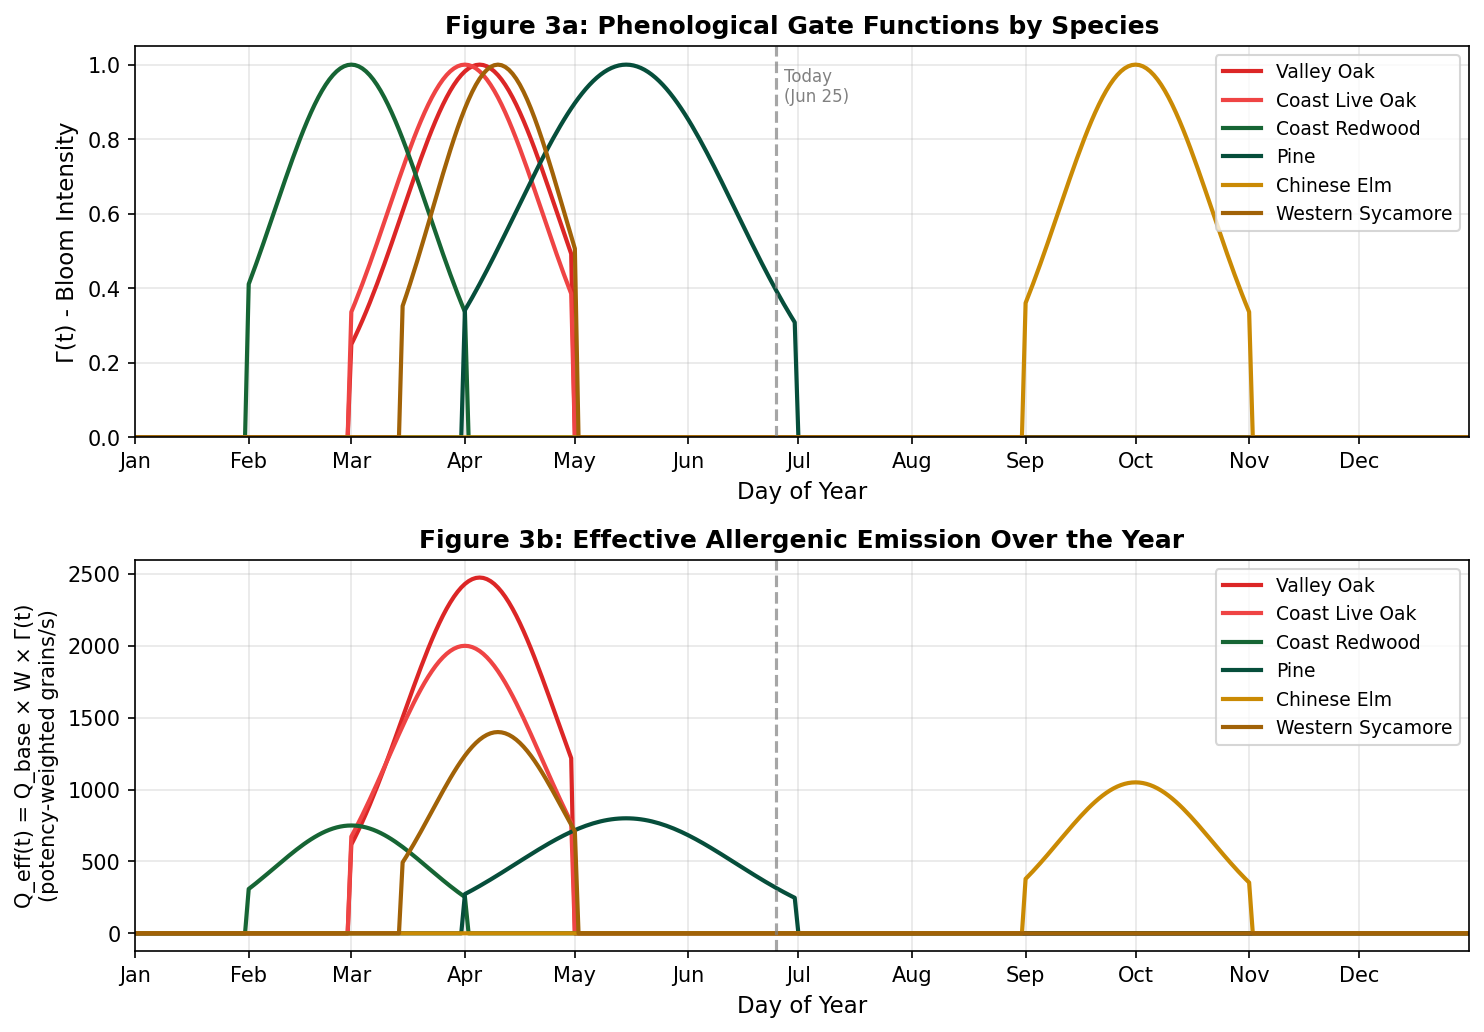
\includegraphics[width=\textwidth]{fig3_phenology.png}
\caption{Phenological emission model. (a) Temporal gate functions $\Gamma_i(t)$ showing blooming intensity across the year for each species. (b) Effective allergenic emission $Q_{eff}(t) = Q_{base} \times W \times \Gamma(t)$. The dashed line marks today (June 25), when most tree species are dormant and only Pine retains weak late-season emission.}
\label{fig:phenology}
\end{figure}

\section{Satellite-Based Vegetation Detection}

\subsection{Image Acquisition}

High-resolution satellite imagery (0.5~m/pixel) is obtained from the Esri World Imagery REST export API, covering the full campus (557~m $\times$ 637~m) at $1600 \times 1398$ pixels.

\subsection{Calibrated Color Segmentation}

Tree canopy pixels are classified using thresholds calibrated from 771 human-verified positive samples:
\begin{equation}
\text{is\_tree} = (g_e > 4) \wedge (35 < \bar{I} < 155) \wedge (r < 165) \wedge (b < 125)
\end{equation}
where $g_e = g - (r+b)/2$ is the green excess and $\bar{I} = (r+g+b)/3$ the mean brightness.

\subsection{Watershed Segmentation}

Adjacent canopies are separated using marker-controlled watershed \citep{beucher1992}:
\begin{enumerate}
    \item Binary mask is eroded (3 iterations) to generate seed markers
    \item Euclidean distance transform computed on the mask
    \item Watershed algorithm segments using inverted distance as elevation
\end{enumerate}

\subsection{Peak-Based Detection}

An alternative pipeline computes a ``tree-ness'' score:
\begin{equation}
S(x,y) = \max(g_e, 0) \cdot \frac{\max(155 - \bar{I}, 0)}{120}
\end{equation}
convolved with a Gaussian ($\sigma = 4$~px). Local maxima with minimum spacing of 7~pixels identify individual tree centers. Canopy radius is estimated from the score falloff profile.

\subsection{Human-in-the-Loop Calibration}

The detection undergoes iterative refinement:
\begin{enumerate}
    \item Automated detection identifies candidates
    \item Users delete false positives via interactive map
    \item Verified positions persist and inform threshold updates
    \item Three rounds achieved $<5\%$ false positive rate
\end{enumerate}

\subsection{Building Rooftop Detection}
\label{sec:buildings}

Building footprints are identified as connected regions satisfying:
\begin{equation}
(\text{saturation} < 30) \wedge (\bar{I} > 160) \wedge (g_e < 8)
\end{equation}
with minimum area 800~pixels ($\approx 20$~m$^2$).

\section{Exposure Assessment}

\subsection{Path-Integrated Dose}

Cumulative exposure along walking path $\gamma$ at speed $v_w = 1.4$~m/s:
\begin{equation}
D = \int_\gamma C_{total}(\mathbf{x}(s)) \cdot \frac{ds}{v_w} \approx \sum_k C(\mathbf{x}_k) \cdot \Delta t_k
\end{equation}

\subsection{Clinical Risk Mapping}

Dose is mapped to actionable risk levels: Low ($D < 50$), Moderate ($50$--$200$), High ($200$--$500$), Very High ($>500$~grain$\cdot$s/m$^3$).

\section{Results}

\subsection{Detection Performance}

After three calibration rounds, the system identifies 1,018 trees: 414 Coast Live Oak, 239 Redwood, 159 Valley Oak, 110 Pine, 76 Sycamore, and 20 Chinese Elm.

\subsection{Seasonal Concentration}

Using a fixed scale (500~grains/m$^3$ = spring peak):
\begin{itemize}
    \item \textbf{April 1} (day 91): $C_{max} = 273$~grains/m$^3$ (55\% of scale); 8 active species
    \item \textbf{June 25} (day 176): $C_{max} = 30$~grains/m$^3$ (6\%); Pine only
    \item \textbf{January} (day 15): $C_{max} \approx 0$; all species dormant
\end{itemize}

\subsection{Spatial Patterns}

The concentration field exhibits: (i) plume elongation along prevailing wind; (ii) zero concentration over building footprints; (iii) enhanced accumulation in building wake zones; (iv) elevated concentrations in oak-dense corridors.

\section{Discussion}

The Gaussian plume approach provides a computationally efficient ($<500$~ms per field computation) approximation suitable for real-time interactive applications. Key limitations include the assumption of spatially uniform wind (neglecting building-channeled flows that would require CFD), the RGB-only species classification (improved with hyperspectral data), and absence of ground-truth pollen measurements for quantitative validation.

The human-in-the-loop calibration workflow drove most of the accuracy gain: automated detection alone achieved approximately 75\% precision, improved to $>95\%$ after three interactive correction rounds. For campus-scale applications, then, semi-automated approaches combining algorithmic detection with targeted human verification are more practical than fully autonomous methods.

The fixed annual scale reveals that allergy risk communication should emphasize seasonal context: a June reading of 30~grains/m$^3$ might alarm students if presented without reference to the 500~grains/m$^3$ spring peak that constitutes the actual high-risk period.

\section{Conclusion}

We built a complete pipeline for hyperlocal pollen dispersion modeling, from satellite-based source identification to physics-based atmospheric transport to path-integrated exposure. The system resolves concentration gradients at 5-meter scale across a 25-hectare campus with 1,018 individually mapped pollen sources and recomputes the full field in under 500~ms as wind and season change. Whether the routes it recommends actually reduce measured exposure is the validation step that remains.

\section*{Data Availability}

The complete source code and campus data are publicly available at \url{https://github.com/jasminejz2021ai/pollenWebApp}. A live, interactive deployment of the system is accessible at \url{https://pollen-web-app-seven.vercel.app/}. The tree inventory is derived from the PAUSD 2009 arborist survey supplemented by satellite detection.

\section*{Acknowledgments}

The author thanks the Palo Alto Unified School District for access to campus tree inventory records.

\begin{thebibliography}{10}

\bibitem[Bousquet et al.(2008)]{bousquet2008}
J.~Bousquet, N.~Khaltaev, A.~A.~Cruz, et al.
\newblock Allergic rhinitis and its impact on asthma (ARIA) 2008 update.
\newblock \emph{Allergy}, 63(S86):8--160, 2008.

\bibitem[Pasquill(1961)]{pasquill1961}
F.~Pasquill.
\newblock The estimation of the dispersion of windborne material.
\newblock \emph{Meteorological Magazine}, 90:33--49, 1961.

\bibitem[Gifford(1961)]{gifford1961}
F.~A.~Gifford.
\newblock Use of routine meteorological observations for estimating atmospheric dispersion.
\newblock \emph{Nuclear Safety}, 2:47--51, 1961.

\bibitem[Turner(1964)]{turner1964}
D.~B.~Turner.
\newblock A diffusion model for an urban area.
\newblock \emph{Journal of Applied Meteorology}, 3(1):83--91, 1964.

\bibitem[Schulman and Scire(1980)]{schulman1980}
L.~L.~Schulman and J.~S.~Scire.
\newblock Buoyant line and point source (BLP) dispersion model user's guide.
\newblock Technical report, Environmental Research and Technology, 1980.

\bibitem[Sofiev et al.(2013)]{sofiev2013}
M.~Sofiev, P.~Siljamo, H.~Ranta, T.~Linkosalo, et al.
\newblock A numerical model of birch pollen emission and dispersion in the atmosphere.
\newblock \emph{Int. J. Biometeorology}, 57:45--58, 2013.

\bibitem[Bastl et al.(2016)]{bastl2016}
K.~Bastl, M.~Kmenta, U.~Berger.
\newblock Defining pollen seasons: background and recommendations.
\newblock \emph{Current Allergy and Asthma Reports}, 18:73, 2016.

\bibitem[Beucher and Meyer(1992)]{beucher1992}
S.~Beucher and F.~Meyer.
\newblock The morphological approach to segmentation: the watershed transformation.
\newblock In \emph{Mathematical Morphology in Image Processing}, pp. 433--481, 1992.

\bibitem[Helbig et al.(2004)]{helbig2004}
N.~Helbig, B.~Vogel, H.~Vogel, F.~Fiedler.
\newblock Numerical modelling of pollen dispersion on the regional scale.
\newblock \emph{Aerobiologia}, 20:3--19, 2004.

\bibitem[PAUSD(2009)]{pausd2009}
Palo Alto Unified School District.
\newblock Gunn High School arborist survey and tree inventory.
\newblock Technical report, PAUSD Facilities Department, 2009.

\end{thebibliography}

\end{document}
